\documentclass[a4paper,12pt]{article} % тип документа
\usepackage[margin=1in]{geometry} % Поля

%  Русский язык
\usepackage[warn]{mathtext}
\usepackage[T2A]{fontenc}			% кодировка
\usepackage[utf8]{inputenc}			% кодировка исходного текста
\usepackage[english,russian]{babel}	% локализация и переносы
% Математика
\usepackage{amsmath,amsfonts,amssymb,amsthm,mathtools} 
\usepackage{wasysym}
%%%
\usepackage{graphicx}

\usepackage{tabularx}

\usepackage{gensymb} % знак градуса
\usepackage{enumitem} % изменить список enumerate
\usepackage{placeins} % \FloatBarrier

\renewcommand{\thesection}{\Roman{section}} 
\renewcommand{\thesubsection}{\roman{subsection}}


\begin{document}

\newcolumntype{Y}{>{\centering\arraybackslash}X} %new tabularx


%титул
\hrule 	
\medskip
\begin{raggedright}
{\large \textbf{Отчёт по работе 5.8.1}}
\\
\medskip
{\Large Определение постоянных Стефана-Больцмана и Планка из анализа теплового излучения накаленного тела} 
\\
\medskip
{\large Карташов Констанин Б04-005}
\medskip
\hrule
\medskip
\end{raggedright}


\section{Анотация}

\paragraph{Цель работы:} 
Измерение температуры модели АЧТ при помощи оптического пирометра и термопары, сравнение получившихся значений. Исследование накалённых тел с различной испускательной способностью. Проверка закона Стефана-Больцмана и получение значений для постоянной Стефана-Больцмана и постоянной Планка.

\paragraph{Оборудование:}
\begin{itemize}
\renewcommand{\labelitemi}{$\triangleright$}
\itemsep0em
\item Оптический пирометр с исчезающей нитью
\item Модель АЧТ с термопарой
\item Трубка с кольцами из веществ с различной испускательной способностью
\item Лампочка накаливания с вольфрамовой нитью
\item Источник питания
\item Вольт- и амперметр
\end{itemize}


\medskip\hrule\medskip

\section{Теоретическая часть}

\paragraph{} В оптической пирометрии различают три температуры: радиационную, цветовую и яркостную. В данной работе используется яркостная температура. Под яркостной температурой понимаю температуру абсолютно чёрного тела, при которой его спектральная испускательная способность равна спектральной испускательной способности исследуемого тела при той же длине волны. 

Измерение яркостной температуры раскалённого тела производится при помощи оптического пирометра с исчезающей нитью. 

\paragraph{} По результатам измерений мощности и излучения вольфрамовой нити можно судить о справедливости закона Стефана-Больцмана. Для этого приравняем мощность потребляемую нитью к излучаемой  ею за единицу времени энергию. Если предположить, что нить излучает как серое тело, то мощностью излучения можно записать в виде:

\[
N = \varepsilon_T S \sigma T^4,
\]

\noindent где $\varepsilon_T$ -- поправочный коэффициент излучения, $S$ -- площадь излучающей поверхности нити, $T$ -- температура нити, $\sigma$ -- постоянная Стефана-Больцмана.

\medskip\hrule\medskip

\section{Экспериментальная часть}

\subsection{Устройство экспериментальной установки}

\begin{figure}[h]
\centering

\includegraphics[width=0.7\textwidth]{setup.png}
\caption{Схема экспериментальной установки}
\label{fig:setup}
\end{figure}

\paragraph{} Экспериментальная установка (рис. \ref{fig:setup}) состоит из: исследуемых образцов (17, 18, 19, 20), источника питания, источника питания, вольтметров и амперметра (14, 15, 17) и пирометра.

\subsection{Изучение работы оптического пирометра}

\paragraph{} Для изучения работы оптического пирометра подключим питание к модели абсолютно чёрного тела. По напряжению на термопаре определим температуру модели АЧТ. Когда температура установиться, измерим температуру модели АЧТ при помощи пирометра и сравним с температурой измеренной при помощи термопары.

Напряжение на термопаре $U_\text{терм} = 42.99$ мВ, температура $T_\text{терм} = 42.99 \textbf{мВ} / 41 \text{мкВ} \approx 1050 \degree$C, учтя температуру комнаты $\approx 20\degree$C получим $T_\text{терм} = 1070 \degree$C. 

Температура измеренная пирометром $T_\text{пиро} = 1089\degree$C, что достаточно близко для того, чтобы считать пирометр исправным.

\subsection{Измерение яркостной температуры накалённых тел}

\paragraph{}Нагреем два металлических кольца до свечения. Так как кольца находятся в контакте, можем считать их температуру одинаковой. При этом мы видим, что свечение у них разного цвета. Из этого можно сделать вывод, что яркостная температура двух тел может различаться при одной и той же действительной температуре.

\subsection{Проверка закона Стефана-Больцмана} 

\paragraph{} Подключим вольфрамовую нить лампы накаливания к источнику питания и направим на неё пирометр. Далее, будем менять напряжение источника питания, и при помощи пирометра измерять соответствующею температуру $T$, при помощи вольтметра и амперметра будем измерять напряжение $U$ и ток $I$ источника питания, исходя из чего найдём мощность $N = UI$ потребляемую лампой. Данные измерений приведены в таблице \ref{tab:exp3}.

\begin{table}[h]
\centering
\begin{tabular}{|l|l|l|l|l|l|l|l|l|}
\cline{1-4} \cline{6-9}
$T$, К & $U$, В & $I$, А & $N$, Вт &  & $T$, К & $U$, В & $I$, А & $N$, Вт \\ \cline{1-4} \cline{6-9} 
1073   & 1.39   & 0.48   & 0.67    &  & 1812   & 5.25   & 0.84   & 4.4     \\ \cline{1-4} \cline{6-9} 
1214   & 1.75   & 0.52   & 0.91    &  & 1869   & 5.62   & 0.87   & 4.87    \\ \cline{1-4} \cline{6-9} 
1265   & 2.13   & 0.56   & 1.2     &  & 1908   & 5.95   & 0.91   & 5.42    \\ \cline{1-4} \cline{6-9} 
1374   & 2.46   & 0.6    & 1.47    &  & 1968   & 6.3    & 0.92   & 5.77    \\ \cline{1-4} \cline{6-9} 
1447   & 2.81   & 0.63   & 1.77    &  & 2005   & 6.65   & 0.94   & 6.26    \\ \cline{1-4} \cline{6-9} 
1519   & 3.17   & 0.66   & 2.11    &  & 2036   & 7.01   & 0.97   & 6.78    \\ \cline{1-4} \cline{6-9} 
1568   & 3.52   & 0.69   & 2.44    &  & 2065   & 7.35   & 0.99   & 7.27    \\ \cline{1-4} \cline{6-9} 
1623   & 3.86   & 0.72   & 2.79    &  & 2082   & 7.72   & 1.01   & 7.84    \\ \cline{1-4} \cline{6-9} 
1653   & 4.2    & 0.75   & 3.16    &  & 2105   & 8.06   & 1.04   & 8.36    \\ \cline{1-4} \cline{6-9} 
1713   & 4.55   & 0.78   & 3.56    &  & 2156   & 8.44   & 1.06   & 8.96    \\ \cline{1-4} \cline{6-9} 
1772   & 4.9    & 0.81   & 3.97    &  & 2178   & 8.83   & 1.09   & 9.61    \\ \cline{1-4} \cline{6-9} 
\end{tabular}
\caption{Даные измерений}
\label{tab:exp3}
\end{table}

\paragraph{} Оценим погрешности данных. В качестве погрешности измерения температуры возьмём $\Delta T = 10$ К (близкие температуры сложно различить пирометром). Погрешность измерения напряжения $\Delta U = 0.01$ В, погрешность измерения силы тока $\Delta I = 0.01$ мА (эти погрешности связаны с флуктуациями показаний вольт- и амперметров). Погрешность в показании мощность вычислим по формуле $\Delta N = N \sqrt{\varepsilon_I^2 + \varepsilon_U^2}$, где $\varepsilon_I$ и $\varepsilon_U$ -- относительные погрешности силы тока и напряжения соответственно.

\paragraph{} Построим график зависимости $\ln N = f(\ln T)$ для проверки закона Стефана-Больцмана (рис. \ref{fig:plot3}). Если зависимость степенная, то на графике должна получиться прямая. $N = \varepsilon_T B T^n, \; \ln N = \ln (\varepsilon_T B) + n \ln T$. Погрешность в логарифмическом масштабе $\ln (\Delta x) = \Delta x / x = \varepsilon_x$ равная относительной погрешности.

\begin{figure}[h]
\centering
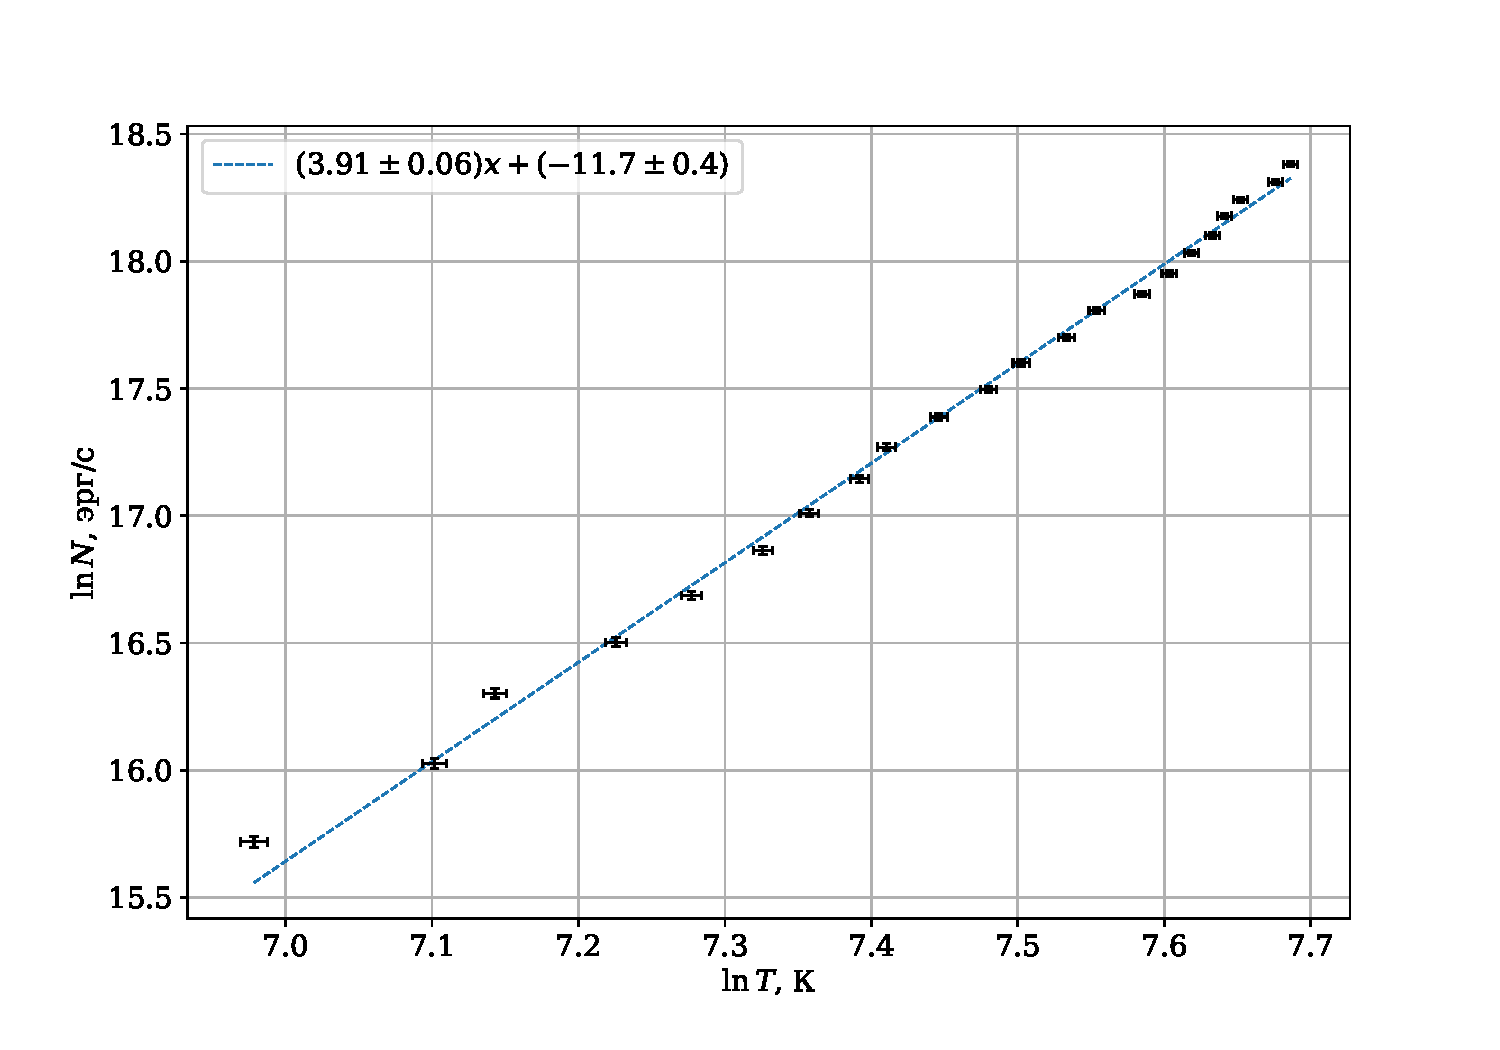
\includegraphics[width=\textwidth]{plot3.pdf}
\caption{Графики зависимости напряжения от температуры в логарифмических координатах}
\label{fig:plot3}
\end{figure}

\paragraph{} Проведём наилучшею прямую через получившиеся точки. Для этого воспользуемся методом наименьших квадратов, в качестве статистического веса точек возьмём величину обратную погрешности логарифма мощности $w = 1/\varepsilon_N$. Получили прямую прямую $y = (3.91 \pm 0.06) x + (-11.7 \pm 0.4)$. То есть $n = 3.91 \pm 0.06$, что достаточно близко к ожидаемому значению.

\subsection{Нахождение постоянных Стефана-Больцмана и Планка}

\paragraph{} Убедившись в состоятельности закона Стефана-Больцмана найдём значение постоянной. Воспользуемся формулой:

\[
\sigma = \frac{N}{\varepsilon_T S T^4}
\]

\noindent для каждого измеренного значения $T$, превышающего 1700 K. Значения для $\varepsilon_T$ возьмём из таблицы 1 в разделе 8 лабораторного практикума. Площадь $S = 0.36$ см$^2$. Погрешность оценим по формуле:

\[
\Delta \sigma = \sigma \sqrt{\left( \frac{\Delta N }{N} \right)^2 + 4\left(  \frac{\Delta T }{T} \right)^2}.
\]

\noindent Получившиеся значения запишем в таблицу \ref{tab:sigma}. По полученным значениям найдём среднее и среднеквадратичную погрешность: $\bar{\sigma} = (4.6 \pm 0.4) \cdot 10^{-5}$ $\frac{\text{эрг}}{\text{см}^2 \text{К}^4 \text{c}}$

\begin{table}[h]
\centering
\scriptsize
\begin{tabular}{|l|c|c|c|c|c|c|c|c|c|c|c|c|c|}
\hline
$T$, К & 1713 & 1772 & 1812 & 1869 & 1908 & 1968 & 2005 & 2036 & 2065 & 2082 & 2105 & 2156 & 2178 \\
\hline
$\sigma$, СГС$\cdot 10^{-5}$ & 5.45 & 5.11 & 5.06 & 4.79 & 4.79 & 4.37 & 4.31 & 4.32 & 4.31 & 4.46 & 4.5 & 4.27 & 4.35 \\
\hline
$\Delta \sigma$, СГС$\cdot 10^{-5}$ & 0.1 & 0.09 & 0.08 & 0.08 & 0.07 & 0.07 & 0.06 & 0.06 & 0.06 & 0.06 & 0.06 & 0.06 & 0.06 \\
\hline
\end{tabular}
\caption{Полученные значения для постоянной Стефана-Больцмана}
\label{tab:sigma}
\end{table}

\paragraph{} Определим значение для постоянной постоянной Планка по формуле:

\[
h = \sqrt{\frac{2 \pi^5 k_\text{Б}^4}{15c^2\sigma}}.
\]

\noindent Проведём расчёт для каждого значения $\sigma$ из таблицы \ref{tab:sigma}, и найдём среднее и среднеквадратичную погрешность: $h = (7.1 \pm 0.2) \cdot 10^{-27}$ эрг$\cdot$с.

\medskip\hrule\medskip

\subsection{Измерение <<яркостной температуры>> неоновой лампочки}

\paragraph{} Подключим неоновую лампочку к источнику питания. Видим что лампочка загорелась красным цветом, соответствующем значению пирометра $T = 900\degree$C. Однако легко убедиться в том, что лампочка холодная. Это можно объяснит тем, что неоновая лампочка излучает свет в дискретном спектре, в отличии от разогретых тел. Этим же эффектом можно объяснить низкую эффективность лапочек накаливания по сравнению со светодиодными и флюоресцентными лампами.

\section{Выводы}

\begin{enumerate}
\item На модели АЧТ проверили работоспособность пирометра.
\item Убедились в том, что у двух разных веществ при одной термодинамической температуре могут быть разные яркостные температуры.
\item Проверили закон Стефана-Больцмана. Увидели, что спектральная излучательная способность пропорциональна температуре в четвёртой степени.
\item Нашли значение постоянной Стефана-Больцмана $\sigma = (4.6 \pm 0.4) \cdot 10^{-5}$ $\frac{\text{эрг}}{\text{см}^2 \text{К}^4 \text{c}}$, что близко к действительному значению $\sigma_\text{теор} = 5.6696 \cdot 10^{-5} \; \frac{\text{эрг}}{\text{см}^2 \text{К}^4 \text{c}}$
\item Нашли значение постоянной Планка  $h = (7.1 \pm 0.2) \cdot 10^{-27}$ эрг$\cdot$с, что близко к действительному значению  $h_\text{теор} = 6.6254 \cdot 10^{-27}$ эрг$\cdot$с.
\item Убедились в том, что для термодинамическая температура неоновой лампочки много меньше яркостной температуры, что объясняется дискретным спектром излучения такой лампочки.
\end{enumerate}



\medskip\hrule\medskip

\end{document}
